\chapter{
Integrating Resource Selection
with
Spatial Capture-Recapture
Models}

\markboth{Resource Selection and Space Usage}{}
\label{chapt.rsf}

\vspace{.3in}

\begin{comment}
Up to this point we have developed many variations of SCR models to
describe the observation process.  These included models of the
relationship between encounter probability and distance, and different
types of covariates such as behavioral responses that can affect
detection probability.  Although these different observation models
are immensely useful, they are rather basic in the sense that they
imply simplistic models of how individuals use space (Sec.
\ref{scr0.sec.implied}) and how individuals are distributed in space.
Here,  we generalize the SCR modeling framework to accommodate more
realistic notions of how animals use space.
\end{comment}


In Chapt. \ref{chapt.scr0} we briefly discussed the notion of how
SCR encounter probability models relate to models of space usage.
When we use symmetric and stationary encounter probability models, SCR
models imply that space usage is a decreasing function of distance
from an individuals home range center. This is not a very realistic
model of space usage in most applications.  In this chapter, we extend SCR
models to incorporate models of resource selection (RS), such as when
one or more explicit landscape covariates are available which the
investigator believes might affect how individual animals use space
within their home range (this is what \citep{johnson:1980} called {\it
  third-order} selection).  Our treatment follows
\citet{royle_etal:2012mee} who integrated a standard family of
resource selection models based on auxilliary telemetry data into the
capture-recapture model for encounter probability, and we reproduce
their case study here, in Sec.
\ref{rsf.chapt.nybears}.
  The extension of SCR models
they proposed is consistent with the manner in which classical
``resource selection function'' (RSF) models \citep{manly_etal:2002}
or utilization distributions \citep{worton:1989, fieberg:2005,
  fieberg:2007} are estimated from animal telemetry data.
\citet{royle_etal:2012mee} argued that SCR models and resource
selection models estimated from telemetry are based on the same basic
underlying model of space usage. The important distinction between SCR
and RSF studies are that, in SCR studies, encounter of individuals is
imperfect (i.e., ``$p<1$'') whereas, with RSF data obtained by
telemetry, encounter is perfect.
We can think of the two as being exactly
equivalent either if we have a dense array of trapping devices, or if
our telemetry apparatus is imperfect such as only samples a small area
of space (this would be consistent with telemetry stations for
sampling fish which only measure passage).


Telemetry studies are extremely common in animal ecology for studying
movement and resource selection, and SCR studies frequently obtain
such data on a subset of individuals. Thus, formal integration of
capture-recapture with telemetry data for the purposes of modeling
resource selection has a number of immediate benefits. For one,
telemetry data provide direct information about $\sigma$
\citep{sollmann_etal:2012ecol,sollmann_etal:inprepjapplecol}. As a
result, this leads to improved estimates of model parameters, and also
has design consequences (see Sec. \ref{design.sec.telemetry}).  In
addition, active resource selection by animals induces a type of
heterogeneity in encounter probability, which is misspecified by
standard SCR encounter probability models. As a result, estimates of
population size or density under models that do not account for
resource selection can be biased \citep{royle_etal:2012mee}.  Finally,
because the resource selection model translates directly to a model
for encounter probability for spatial capture-recapture data, the
implication of this is that it allows us to estimate resource
selection model parameters directly from SCR data, i.e., {\it absent}
telemetry data. This fact should broaden the practical relevance of
spatial capture-recapture for studying or estimating not just density,
but also for directly studyin movement and resource selection.

Telemetry data has been widely used in conjuncation with
capture-recapture data.  For example, \citet{white_shenk:2001} and
\citet{ivan:2012} suggested using telemetry data to estimate the
probability that an individual is exposed to sampling. However, their
estimator requires that individuals are sampled in proportion to this
unknown quantitiy, which seems impossible to acheive in many
studies. In addition, they do not directly integrate the telemetry
data with the capture-recapture model so that common parameters are
jointly estimated.  \citet{sollmann_etal:inprepjapplecol} and
\citet{sollmann_etal:2012ecol} used telemetry data to directly inform
the parameter $\sigma$ from the bivariate normal SCR model in order to
improve estimates of density, although these models did not include an
explicit resource selection component.



%%% one idea is to use these models to account for sampling along
%%% trails.
%%% define z(x) = trail density or average distance to trail




\section{A Model of Space Usage}
\label{rsf.sec.rsfmodel}


Assume that the landscape is defined in terms of a discrete raster of
one or more covariates, having the same dimensions and extent.  Let
${\bf x}_{1},\ldots,{\bf x}_{nG}$ identify the center coordinates of
$nG$ pixels that define a landscape.  We organize these coordinates
into the matrix ${\bf X}_{nG \times 2}$.  Let $C({\bf x})$ denote a
covariate measured (or defined) for every pixel ${\bf x}$.  We suppose
that individual members of some population wander around space in some
manner related to the covariate $C({\bf x})$.
%We will define ``use
%of ${\bf x}$'' to be the event that an individual animal appeared in
%some pixel ${\bf x}$ during some prescribed, but arbitrary, time
%interval. Truth
%therefore exists, at least as it
%relates to space usage by an individual.

As a biological matter, use is the outcome of individuals moving
around their home range \citep{hooten_etal:2010}, i.e., where an
individual is at any point in time is the result of some movement
process. However, to understand space usage, it is not necessary to
entertain explicit models of movement, just to observe the outcomes,
and so we don't elaborate further on what could be sensible or useful
models of movement, but we imagine existing methods of hierarchical or
state-space models are suitable for this purpose
\citep{ovaskainen:2004, jonsen_etal:2005, forester_etal:2007,
  ovaskainen_etal:2008, patterson_etal:2008, hooten_etal:2010,
  mcclintock_etal:2012}.  We consider explicit movement models in the
context of SCR models later chapters of this book
(Chapts. \ref{chapt.search-encounter} and \ref{chapt.open}).  Here we
adopt more of a phenomenological formulation of space usage as
follows: If an individual moves from a pixel ${\bf x}$ to another
pixel ${\bf x}'$, this is defined as a decision to ``use'' pixel ${\bf
  x}'$. This also induces a definition of ``truth'' -- that is, over
any prescribed time interval, the animals makes some number, say $R$
of use decisions, and they are, conceivably, observable by some
omnipotent accounting mechanism (e.g., continuous telemetry).
%%%%  XXX need to check notation consistent with chapter 5 XXXX
%%% There , , ,  we use "m" for true use frequency, so this is good
In this
case, let $m_{ij}$ be the {\it true} use frequency of pixel $j$ by
individual $i$ -- i.e., the number of times individual $i$ used pixel
$j$.  We assume the vector of use frequencies ${\bf m}_{i} =
(m_{i1},\ldots,m_{iG})$ has a multinomial distribution:
\[
{\bf m}_{i} \sim \mbox{Multinomial}(M_{i}, {\bm \pi}_{i})
\]
where $m_{i.} = \sum_{j} m_{ij}$ is the total number of ``use decisions''
made by individual $i$ and
\[
 \pi_{ij} = \frac{ \exp( \alpha_{2} C({\bf x}_{j}) ) }{ \sum_{x}
   \exp(\alpha_{2} C({\bf x}))}
\]
This is a standard RSF model \citep{manly_etal:2002} used to model
telemetry data. In particular, this is ``protocol A'' of
\citep{manly_etal:2002} where all available pixels are censused, and
used pixels are sampled randomly for each individual.
\begin{comment}
One thing about Manly et al 2002 is that they offer
  numerous ways of modeling resource selection. They offer three
  ``protocols'' (pg 5) describing how used and unused resources are
  sampled. What we are discussing is their protocol A where all
  available resources (pixels) are censused, and used pixels are
  sampled randomly for each individual. They also describe 3 designs
  that vary in whether or not individual level data is collected. I
  think it is just worth being aware of this stuff because everybody
  that talks about RSFs thinks in these terms.
\end{comment}
The parameter $\alpha_2$ is the effect of the
landscape covariate $C({\bf x})$ on the relative probability of
use. Thus, if $\alpha_2$ is positive, the relative probability of use
increases as the covariate increases.

In practice, we don't get to observe $m_{ij}$ for all individuals but,
instead, only for a small subset which we capture and install
telemetry devices on.  For the telemetered individuals, we assume
their behavior is according to the same RSF model as the population as
a whole.  To extend this model to make it more realistic, and
consistent with the formulation of SCR models, let ${\bf s}$ denote
the centroid of an individuals home range and let $d_{ij} = ||{\bf
  x}_{j} - {\bf s}_{i}||$ be the distance from the home range center
of individual $i$, ${\bf s}_{i}$, to pixel $j$, ${\bf x}_{j}$. We
modify the space usage model to accommodate that space use will be
concentrated around an individuals home range centroid:
\begin{equation}
 \pi_{ij} = \frac{ \exp( -\alpha_{1} d_{ij}^{2} +\alpha_{2} C({\bf x}_{j}) ) }
{ \sum_{x} \exp(-\alpha_{1} d_{ij}^{2} +\alpha_{2} C({\bf x}_{j}))}
\label{rsf.eq.rsf}
\end{equation}
where $\alpha_1=1/(2\sigma^2)$ describes the rate at which capture
probability declines as a function of distance.  The parameters
$\alpha_{1}$, $\alpha_{2}$ and the activity centers ${\bf s}$ can be
estimated directly from standard telemetry data, using standard
likelihood methods based on the multinomial likelihood
\citep{johnson_etal:2008}.
%We note that this form
%(Eq. \ref{rsf.eq.rsf}) arises explicitly as a limiting form of the
%Gaussian process movement model of
%\citet{johnson_etal:2008}. C
The model Eq.~\ref{rsf.eq.rsf} can be understood as a compound model
of space usage governed by distance-based ``availability'' according
to a Gaussian kernel, and also ``use'', conditional on availability
\citep{johnson_etal:2008, forester_etal:2009}.  Further,
Eq.~\ref{rsf.eq.rsf} resembles standard SCR encounter probability
models that we have used previously, but here with an additional
covariate $C({\bf x})$ (and see Chapt. \ref{chapt.poisson-mn}).  In
particular, under this model for space usage or resource selection, if
we have no covariates at all, or if $\alpha_{2} = 0$, then the
probabilities $\pi_{ij}$ are directly proportional to the SCR model
for encounter probability.  That is, setting $\alpha_{2} = 0$, then
the probability of use for pixel $j$ is:
\[
p_{ij} \propto  \exp( -\alpha_{1} d_{ij}^{2}).
\]
Clearly, whatever function of distance we use in the RSF model implies
an equivalent model of space usage (Sec. \ref{scr0.sec.implied}) as an
SCR model for encounter probability.  In particular, for whatever
model we choose for $p_{ij}$ in an ordinary SCR model, we can modify
the distance component in the RSF function in Eq. \ref{rsf.eq.rsf}
accordingly to be consistent with that model, by using whatever
function $p_{ij}$ we choose according to
\[
\pi_{ij} \propto \exp( \log(p_{ij}) + \alpha_{2} C({\bf x}_{j}) )
\]
(see \citep{forester_etal:2009}).
One difference between this observation model and those that we have
considered in previous chapters is that it includes the normalizing
constant $\sum_{x} \exp(-\alpha_{1} d_{ij}^{2} +\alpha_{2} C({\bf
  x}_{j}))$, which ensures that the use distribution is a proper
probability density function. Thus we are able to characterize the
probability of encounter in terms of both distance and space use.

\citet{royle_etal:2012mee} have a figure showing some typical space
usage patterns under this model, for a simulated covariate, which we
reproduce here in Fig.~\ref{rsf.fig.homeranges}.
\begin{figure}[ht]
\centering
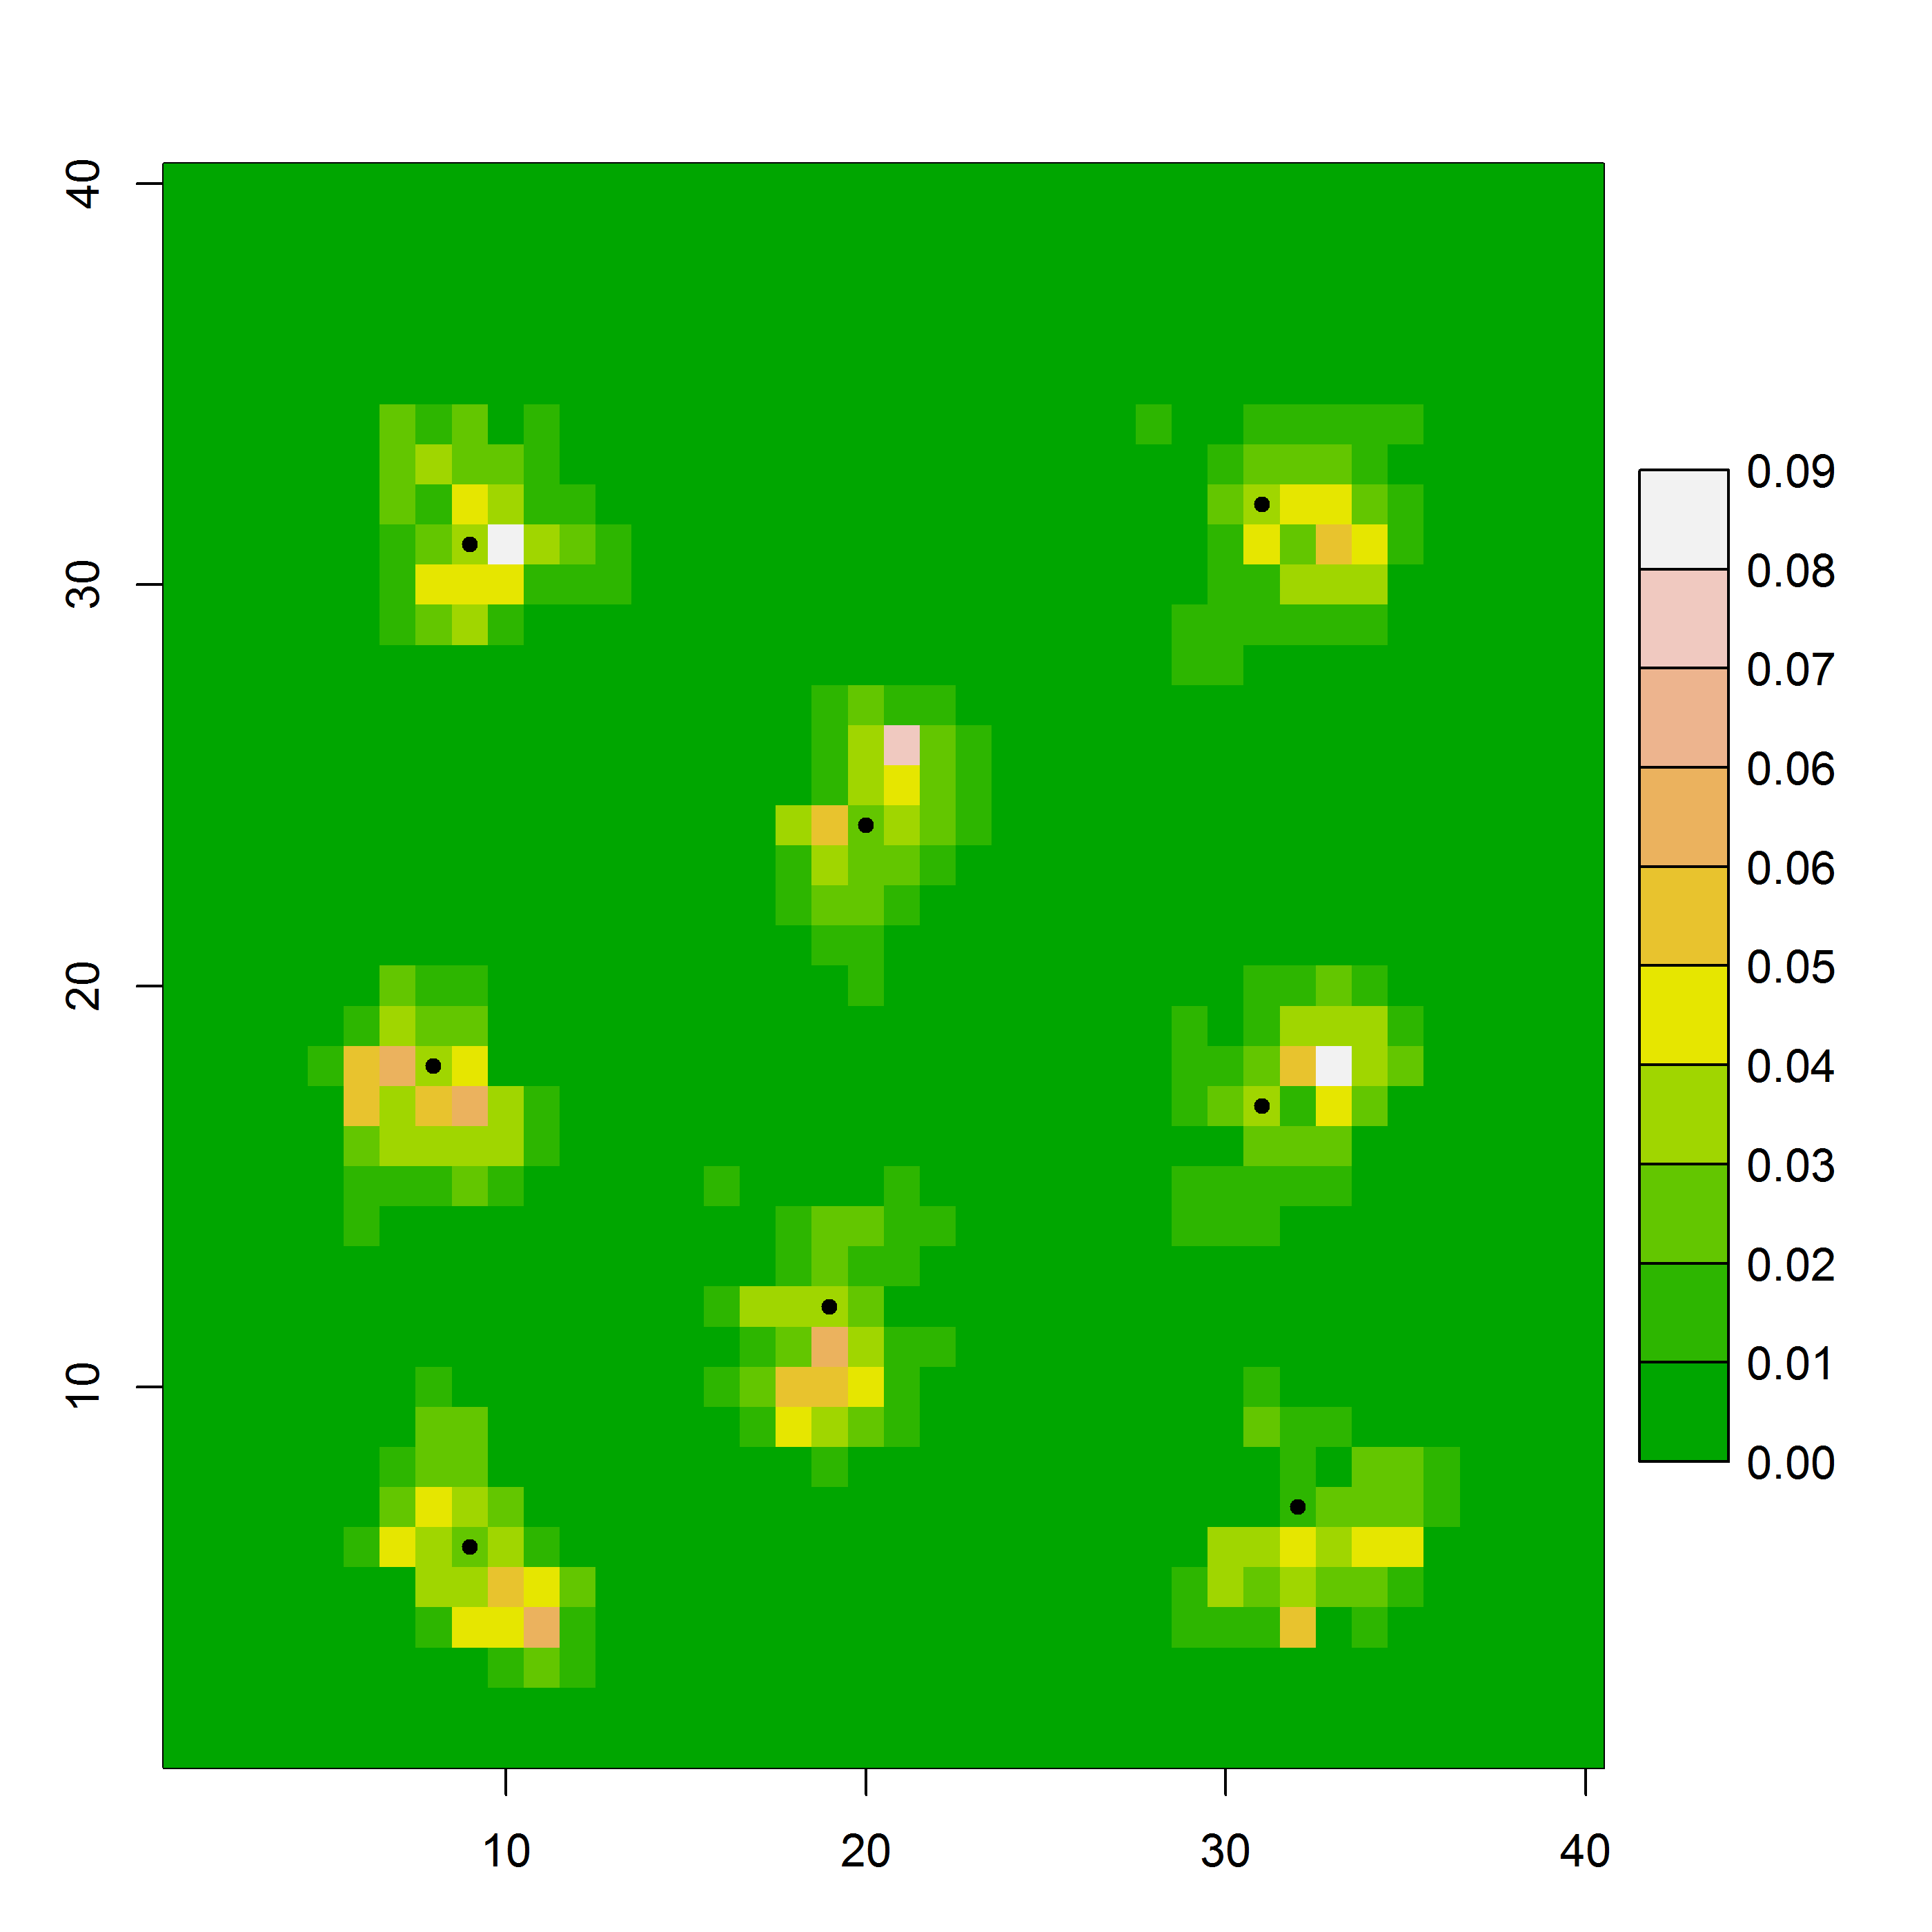
\includegraphics[width=3.5in,height=3.5in]{Ch13-RSF/figs/homeranges8}
\caption{Space usage patterns of 8 individuals under a space usage
  model that contains a single covariate (shown in
  Fig. \ref{rsf.fig.habitat}). Plotted value is the multinomial
  probability $\pi_{ij}$ for pixel $j$ under the model in Eq. \ref{rsf.eq.rsf}.
}
\label{rsf.fig.homeranges}
\end{figure}
These home ranges were simulated
with $\alpha_{1} =
1/(2\sigma^2)$ with $\sigma = 2$ and the coefficient on $C({\bf x})$
set to $\alpha_{2} = 1$.
The covariate in this case was simulated by using a kriging
interpolator with the following {\bf R} commands:
\begin{verbatim}
> set.seed(1234)
> gr <- expand.grid(1:40,1:40)
> Dmat<-as.matrix(dist(gr))
> V <- exp(-Dmat/5)
> z <- t(chol(V))%*%rnorm(1600)
\end{verbatim}
These space usage densities -- ``home ranges'' -- exhibit clear
non-stationarity in response to the structure of the underlying
covariate, and they are distinctly asymmetrical.  We note that if
$\alpha_{2}$ were set to 0, the 8 home ranges shown here would
be proportional to bivariate normal kernels with $\sigma = 2$.
These commands, and those to produce Fig. \ref{rsf.fig.habitat} are in
the package \mbox{\tt scrbook} (see \mbox{\tt ?RSF\_example}).
\begin{figure}[ht]
\centering
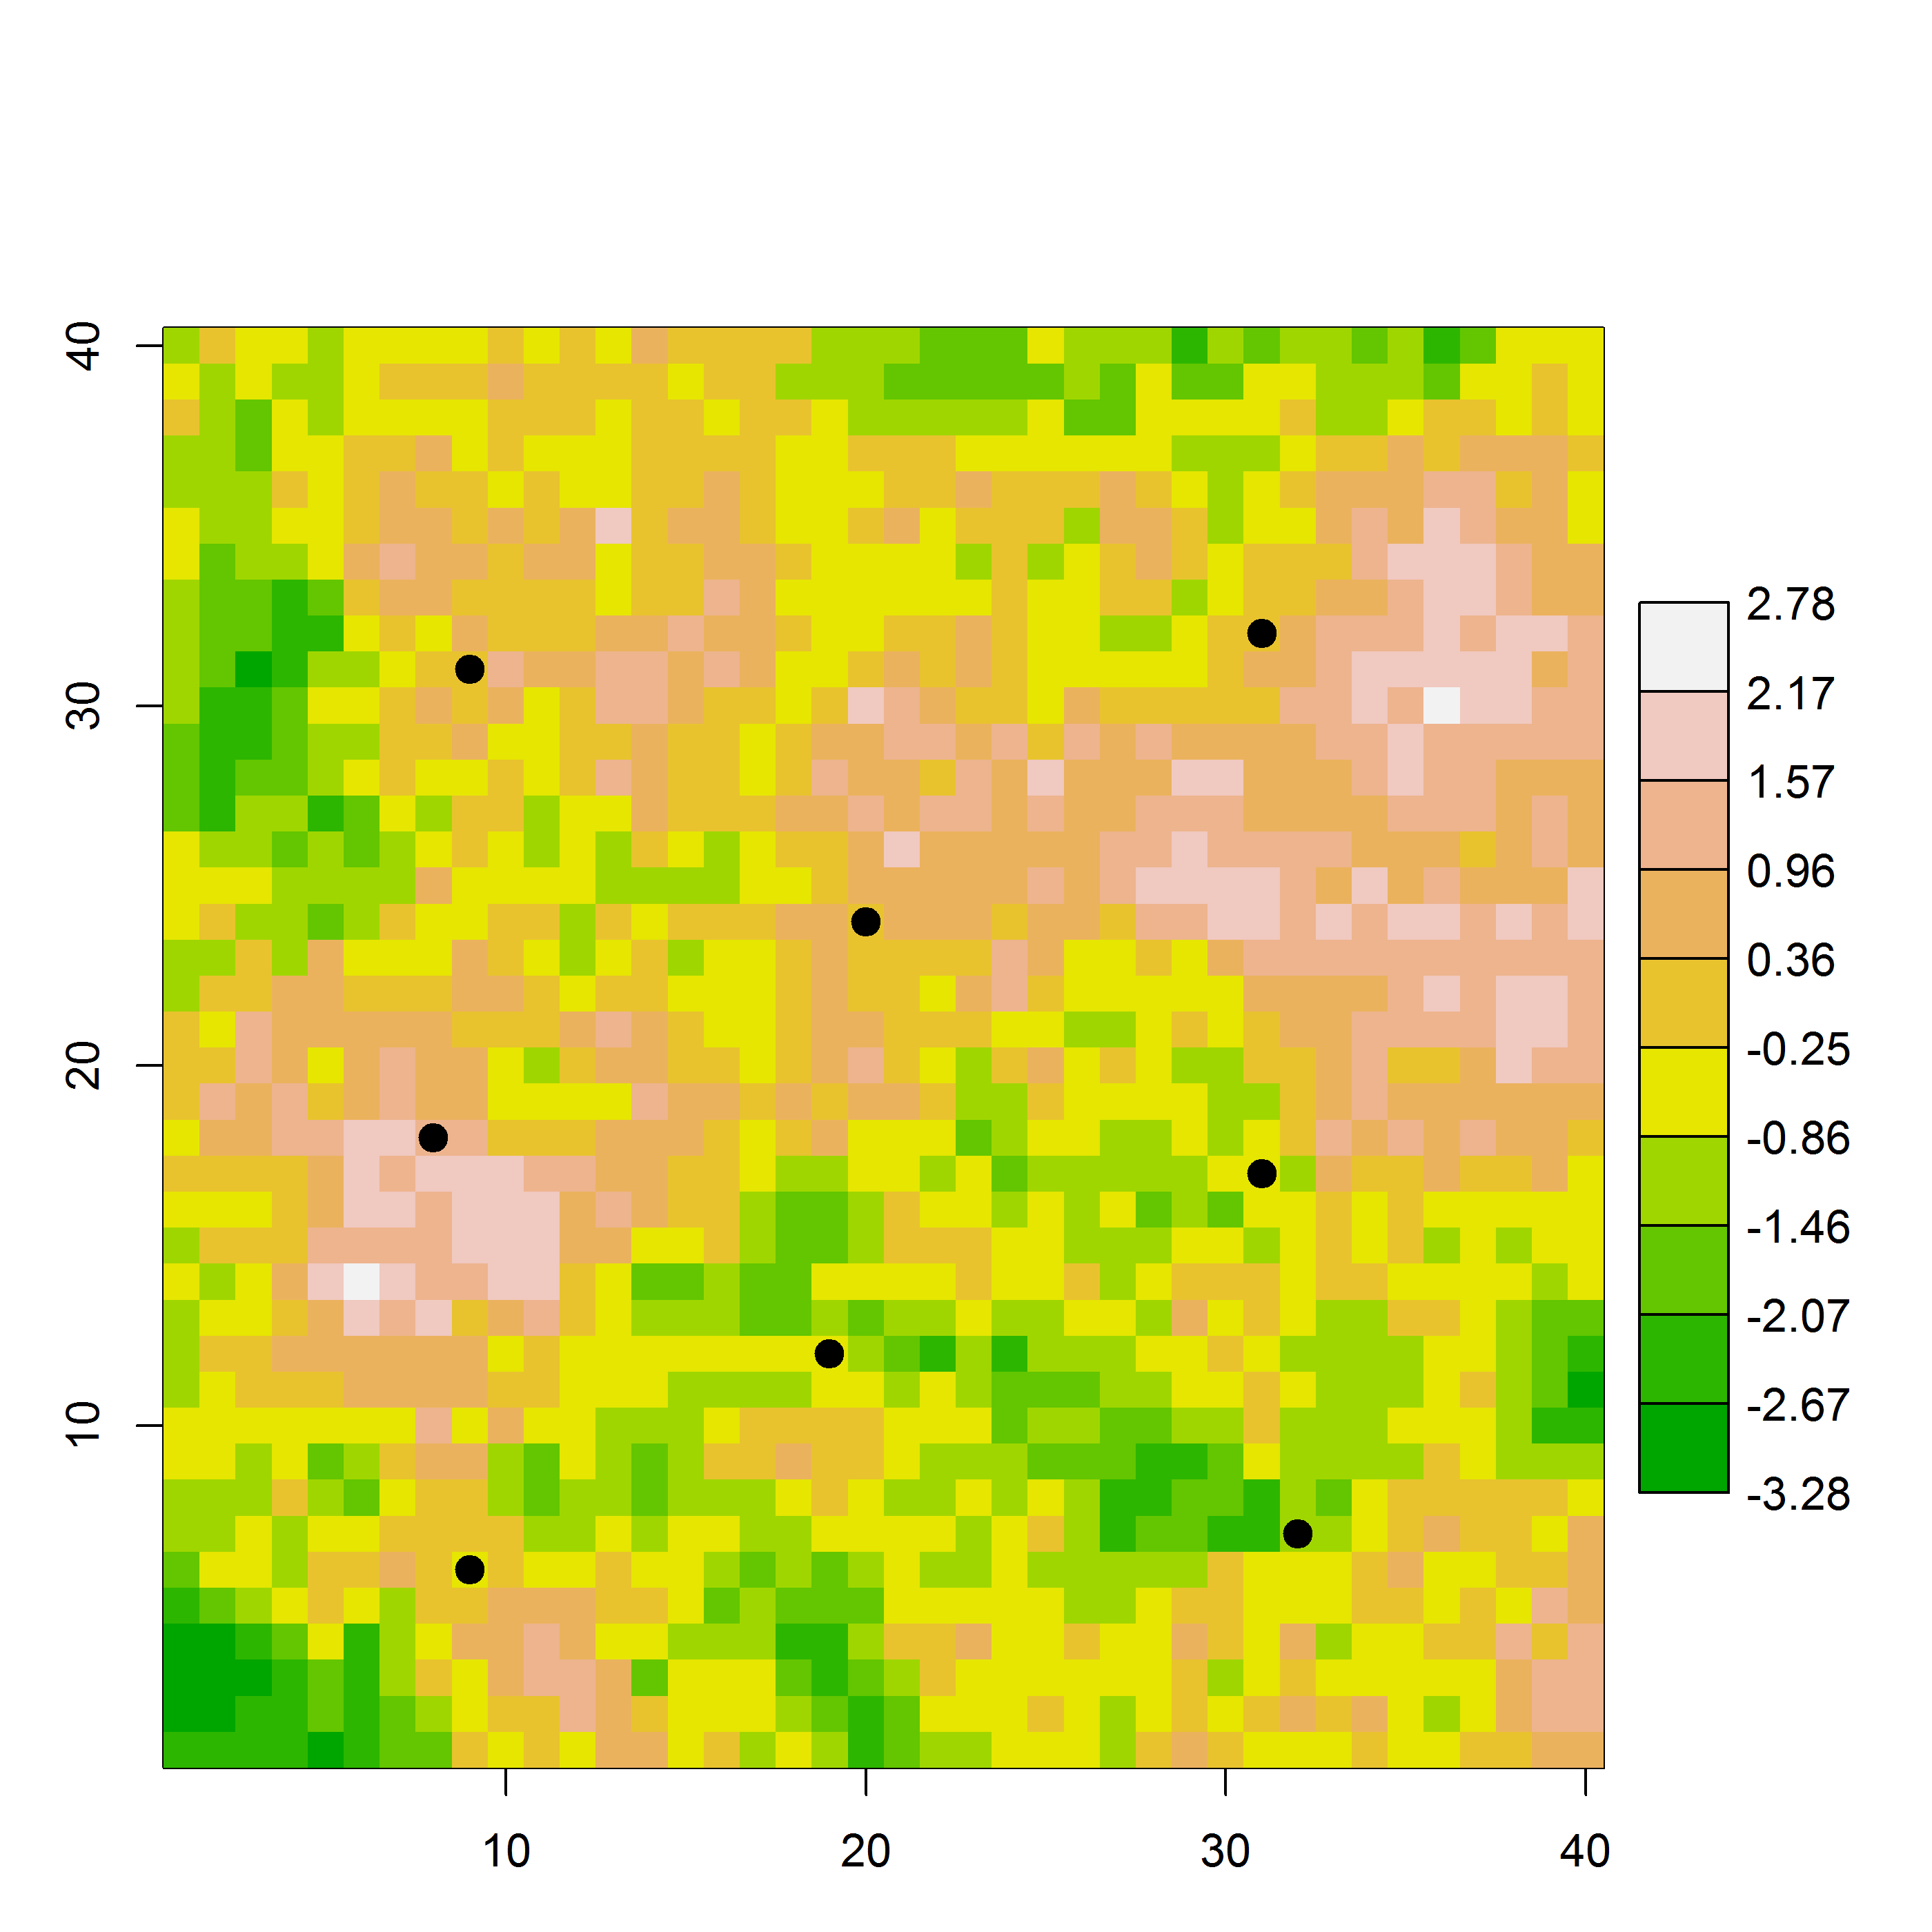
\includegraphics[width=3.15in,height=2.93in]{Ch13-RSF/figs/habitat.png}
\caption{A typical habitat covariate reflecting habitat quality or
  hypothetical utility of the landscape to a species under study. Home
  range centers for 8 individuals are shown with black dots.}
\label{rsf.fig.habitat}
\end{figure}


\subsection{Poisson use model}

A natural way to motivate the multinomial model of space usage is to
assume that individuals make a sequence of resource selection
decisions so that the outcomes $m_{ij}$ are marginally {\it
  independent}, having a Poisson distribution:
\[
 m_{ij} \sim \mbox{Poisson}( \lambda_{ij})
\]
where
\[
 \log(\lambda_{ij}) = \alpha_{0} -\alpha_{1} d_{ij}^{2} +  \alpha_{2} C({\bf x})
\]
In this case, the number of visits to any particular cell is affected
by the covariate $C({\bf x})$ but has a baseline rate ($\exp(\alpha_{0})$)
related to the amount of movement occuring over some time interval.
This is an equivalent model to the multinomial model given previously
in the sense that, if we condition on the total sample size $m_{i.} =
\sum_{j} m_{ij}$, then the vector ${\bf m}_{i}$ has a multinomial
distribution with probabilities given by Eq. \ref{rsf.eq.rsf} (see
also Chapt. \ref{chapt.poisson-mn}).  Also note that if use
frequencies are summarized over individuals for each pixel, i.e.,
create the totals $m_{j.} = \sum_i m_{ij}$, then a standard Poisson
regression model for the resulting ``quadrat counts'' is
reasonable. This is ``Design I'' in \citet{manly_etal:2002}.

In practice, we never observe ``truth'', i.e., the actual use
frequencies $m_{ij}$. Instead, we observe a sampling of the actual use
outcomes by an individual.  As formulated in
Sec. \ref{scr0.sec.implied}, we assume a binomial (``random'')
sampling model:
\[
 y_{ij} \sim \mbox{Binomial}(m_{ij}, p_{0}).
\]
We can think of these counts as arising by thinning the underlying
point process (here, aggregated into pixels) where $p_{0}$ is the
thinning rate of the point process.  In this case, the marginal
distribution of the observed counts $y_{ij}$ is also Poisson but with mean
\[
 \log(\mathbb{E}(y_{ij}))  = \log(p_{0}) + \alpha_{0} -\alpha_{1} d_{ij}^{2} +  \alpha_{2} C({\bf x}).
\]
Thus, the space-usage model (RSF) for the thinned counts $y_{ij}$ is
the same as the space-usage model for the original variables $m_{ij}$.
This is because if we remove $m_{ij}$ from the conditional model by
summing over its possible values, then the vector of ${\bf y}_{i}$ is
{\it also} multinomial with cell probabilities
\[
\pi_{ij} = \frac{p_{0}\lambda_{ij}}{\sum_{j} p_{0} \lambda_{ij}}
\]
and so the nuisance parameter $p_{0}$, indeed the effective intercept
$\log(p_{0}) + \alpha_{0}$, cancels from the numerator and
denominator. Thus, the underlying RSF model applies to the true
unobserved count frequencies ${\bf m}_{i}$ and also those produced
from thinning or sampling, ${\bf y}_{i}$.

%KEY POINT LOST HERE IS THAT BOTH TELEMETRY AND SCR ARE RANDOMLY
%THINNED VERSIONS OF THE POINT PROCESS, PROVIDED CAMERA TRAPPING IS
%RANDOM ALSO

In summary, if we conduct a telemetry study we observe ${\bf m}_{i}$,
the $nG \times 1$ vector of pixel-counts for each individual
$i=1,\ldots,N_{tel}$.
%We declare these data to be
%``resource-selection data'' which are typical of the type used to
%estimate resource-selection functions (RSFs) \citep{manly_etal:2002}.
Sometimes in RSF modeling activities we might have continuous
covariates and so the denominator in Eq. \ref{rsf.eq.rsf} involves an
integration over a distribution for the covariate which is the
conditional intensity of observed point locations in a point process
model. However, in a discrete landscape, entertaining pdfs for the
covariates isn't necessary \citep{royle_etal:2012mee} when we
recognize that the denominator should be the expectation over {\it
  space} and not the pdf of some covariate.


\section{Integrating Capture-Recapture Data}

{\bf XXXXXXXXXXXXXXXXXXX
RC says: After reconciling SCR and RSF, cite that paper
by Boyce and McDonald where they try to do accomplish the same
objective using ad-hoc methods. That is the only effort to do
something similar that I am aware of.
XXXXXXXXXXXXXXXXXXXXXXXXXX
Andy says: I think the idea they had is potentially interesting. Their Pr(s)
distribution
might be the average conditional-on-s RSF, is it a valid estimate of
relative density?
}

The key to combing RSF data with SCR data is to formulate SCR models
in terms of the underlying model of space usage that we just
developed. That is, as if the resulting encounter (in a trap) is the
result of some thinning of the ``true'' space usage outcomes.
%We can
%define the true use frequency for each pixel as an intermediate
%latent variable to which both telemetry data and SCR data are linked.
%Obviously we have to assume that both telemetered individuals and SCR
%individuals are using space according to the same resource selection
%model.
%The difference is that, for SCR data, we do not have sampling
%devices in all locations (pixels) in the landscape, and hence the data
%are only recorded at a subsample of them.
%XXXXX {\bf move the
%  following } XXXXX
In other words, imagine that we have a sampling
device, such as a camera trap, in {\it every} pixel. If the device
operates continually then it is no different from a telemetry
instrument.  If it operates intermittently, or does not expose the
entire area of each pixel, then a reasonable model for this imperfect
observation is the ``thinned'' binomial model given above, where
$\lambda_{0} \equiv \exp(p_{0})$ represents the sampling
effectiveness of the device. So we imagine that the hypothetical
perfect data from a camera trapping study are the thinned counts
$y_{ij}$ for every pixel $j$.

Sampling by SCR produces either Poisson counts $y_{ij}$ or Bernoulli
encounters depending on the type of sampling being done. For example,
a Poisson sampling model
\[
y_{ij} \sim \mbox{Poisson}(\lambda_{0} \lambda_{ij})
\]
or if the observations are binary,
where $y_{ij} = 1$ if the individual $i$ visited
the pixel containing a trap and was detected, then we imagine that
$y_{ij}$ is related to the latent variable $m_{ij}$ being the event
$m_{ij}>0$, which occurs with probability
\[
 p_{ij} = 1-\exp(- \lambda_{0} \lambda_{ij})
\]
%We combine the constants so that $\alpha_{0} = \log(\lambda_{0}) + a_{0}$
%is the baseline encounter rate which includes the constant intensity
%of use by the individual and also the baseline rate of detection,
%conditional on use.  The Bernoulli observation model implies that the
and then the observed encounter frequencies for individual $i$ and trap $j$, from
sampling over $K$ occassions is:
\[
 y_{ij}|{\bf s}_{i} \sim \mbox{Binomial}(K; p_{ij})
\]

A key point here is that if resource selection is happening, then it
appears as a covariate on encounter rate (or encounter
probability), in the same way as ordinary covariates we discussed in
Chapt. \ref{chapt.covariates}.


\subsection{The Joint RSF/SCR Likelihood}

To construct the likelihood for SCR data when we have auxiliary
covariates on space usage {\it or} direct information on space usage
from telemetry data, we regard the two samples (SCR and RSF) as
independent of one another.

Regarding the two data sets as being independent, our approach here
is to form the likelihood for each set of observations as a function
of the same underlying parameters and then combine them. In
particular, let ${\cal L}_{scr}(\alpha_{0}, \alpha_{1}, \alpha_{2}, N;{\bf y}_{scr})$
be the likelihood for the SCR data in terms of the basic encounter
probability parameters and the total (unknown) population size $N$,
and let ${\cal L}_{rsf}(\alpha_{1},\alpha_{2}; {\bf m}_{rsf})$ be the
likelihood for the RSF data based on telemetry which, because the
sample size of such individuals is fixed, does not depend on $N$.
Assuming independence of the two datasets, the
joint likelihood is the product of these two pieces:
\[
{\cal L}_{rsf+scr}(\alpha_{0},\alpha_{1},\alpha_{2},N; {\bf y}_{scr},{\bf
  m}_{rsf})  =
{\cal L}_{scr}(\alpha_{0}, \alpha_{1}, \alpha_{2}, N;{\bf y}_{scr})
\times
{\cal L}_{rsf}(\alpha_{1},\alpha_{2}; {\bf m}_{rsf})
\]
Where the ${\cal L}_{scr}$ is the standard integrated likelihood
(Chapt. \ref{chapt.mle}), and the RSF likelihood contribution is the
multinomial telemetry likelihood having cell probabilities
Eq. \ref{rsf.eq.rsf}.  The {\bf R} code for this was given in the
supplement to \citet{royle_etal:2012mee}, and we include a version of
this in the \mbox{\tt scrbook} package, see \mbox{\tt ?intlik3rsf},
which also shows how to simulate data and fit the combined SCR+RSF
model.



\section{Application: New York Black Bear Study}
\label{rsf.chapt.nybears}

\citet{royle_etal:2012mee} applied the integrated SCR+RSF model to
data from a study of black bears in a region of approximately 4,600
km$^2$ in southwestern New York \citep{sun:2013}\footnote{This is
different from our Fort Drum bear study data set which we've analyzed
in previous chapters}. We reproduce their
main results here.  The data can be loaded from the \mbox{\tt scrbook}
library with the command \mbox{\tt data(nybears)}.

The data are based on a noninvasive, genetic, mark-recapture study
using 103 hair snares in June and July, 2011.  Hair snares were baited
and scented and checked weekly for hair \citep{sun:2013}.  The study
yielded relatively sparse encounter histories
 of 33 individuals and a total of 14 recaptures (27
individuals captured 1 time only;
 Extra trap recaptures included
3 individuals captured in 2 traps, 1 individual in each of 3 and 4
traps).  Data were available for 3 radio-telemetered individuals.
Radio fixes were obtained approximately once per hour, but this was
thinned to once per 10 hours to produce movement outcomes that might
be more independent. This produced 195 telemetry locations used in the
RSF component of the model.  The covariate used in the modeling is
elevation, a standardized version of which is shown in
Fig. \ref{fig.elevation}. This shows also the locations of each
capture.

\begin{figure}
\centering
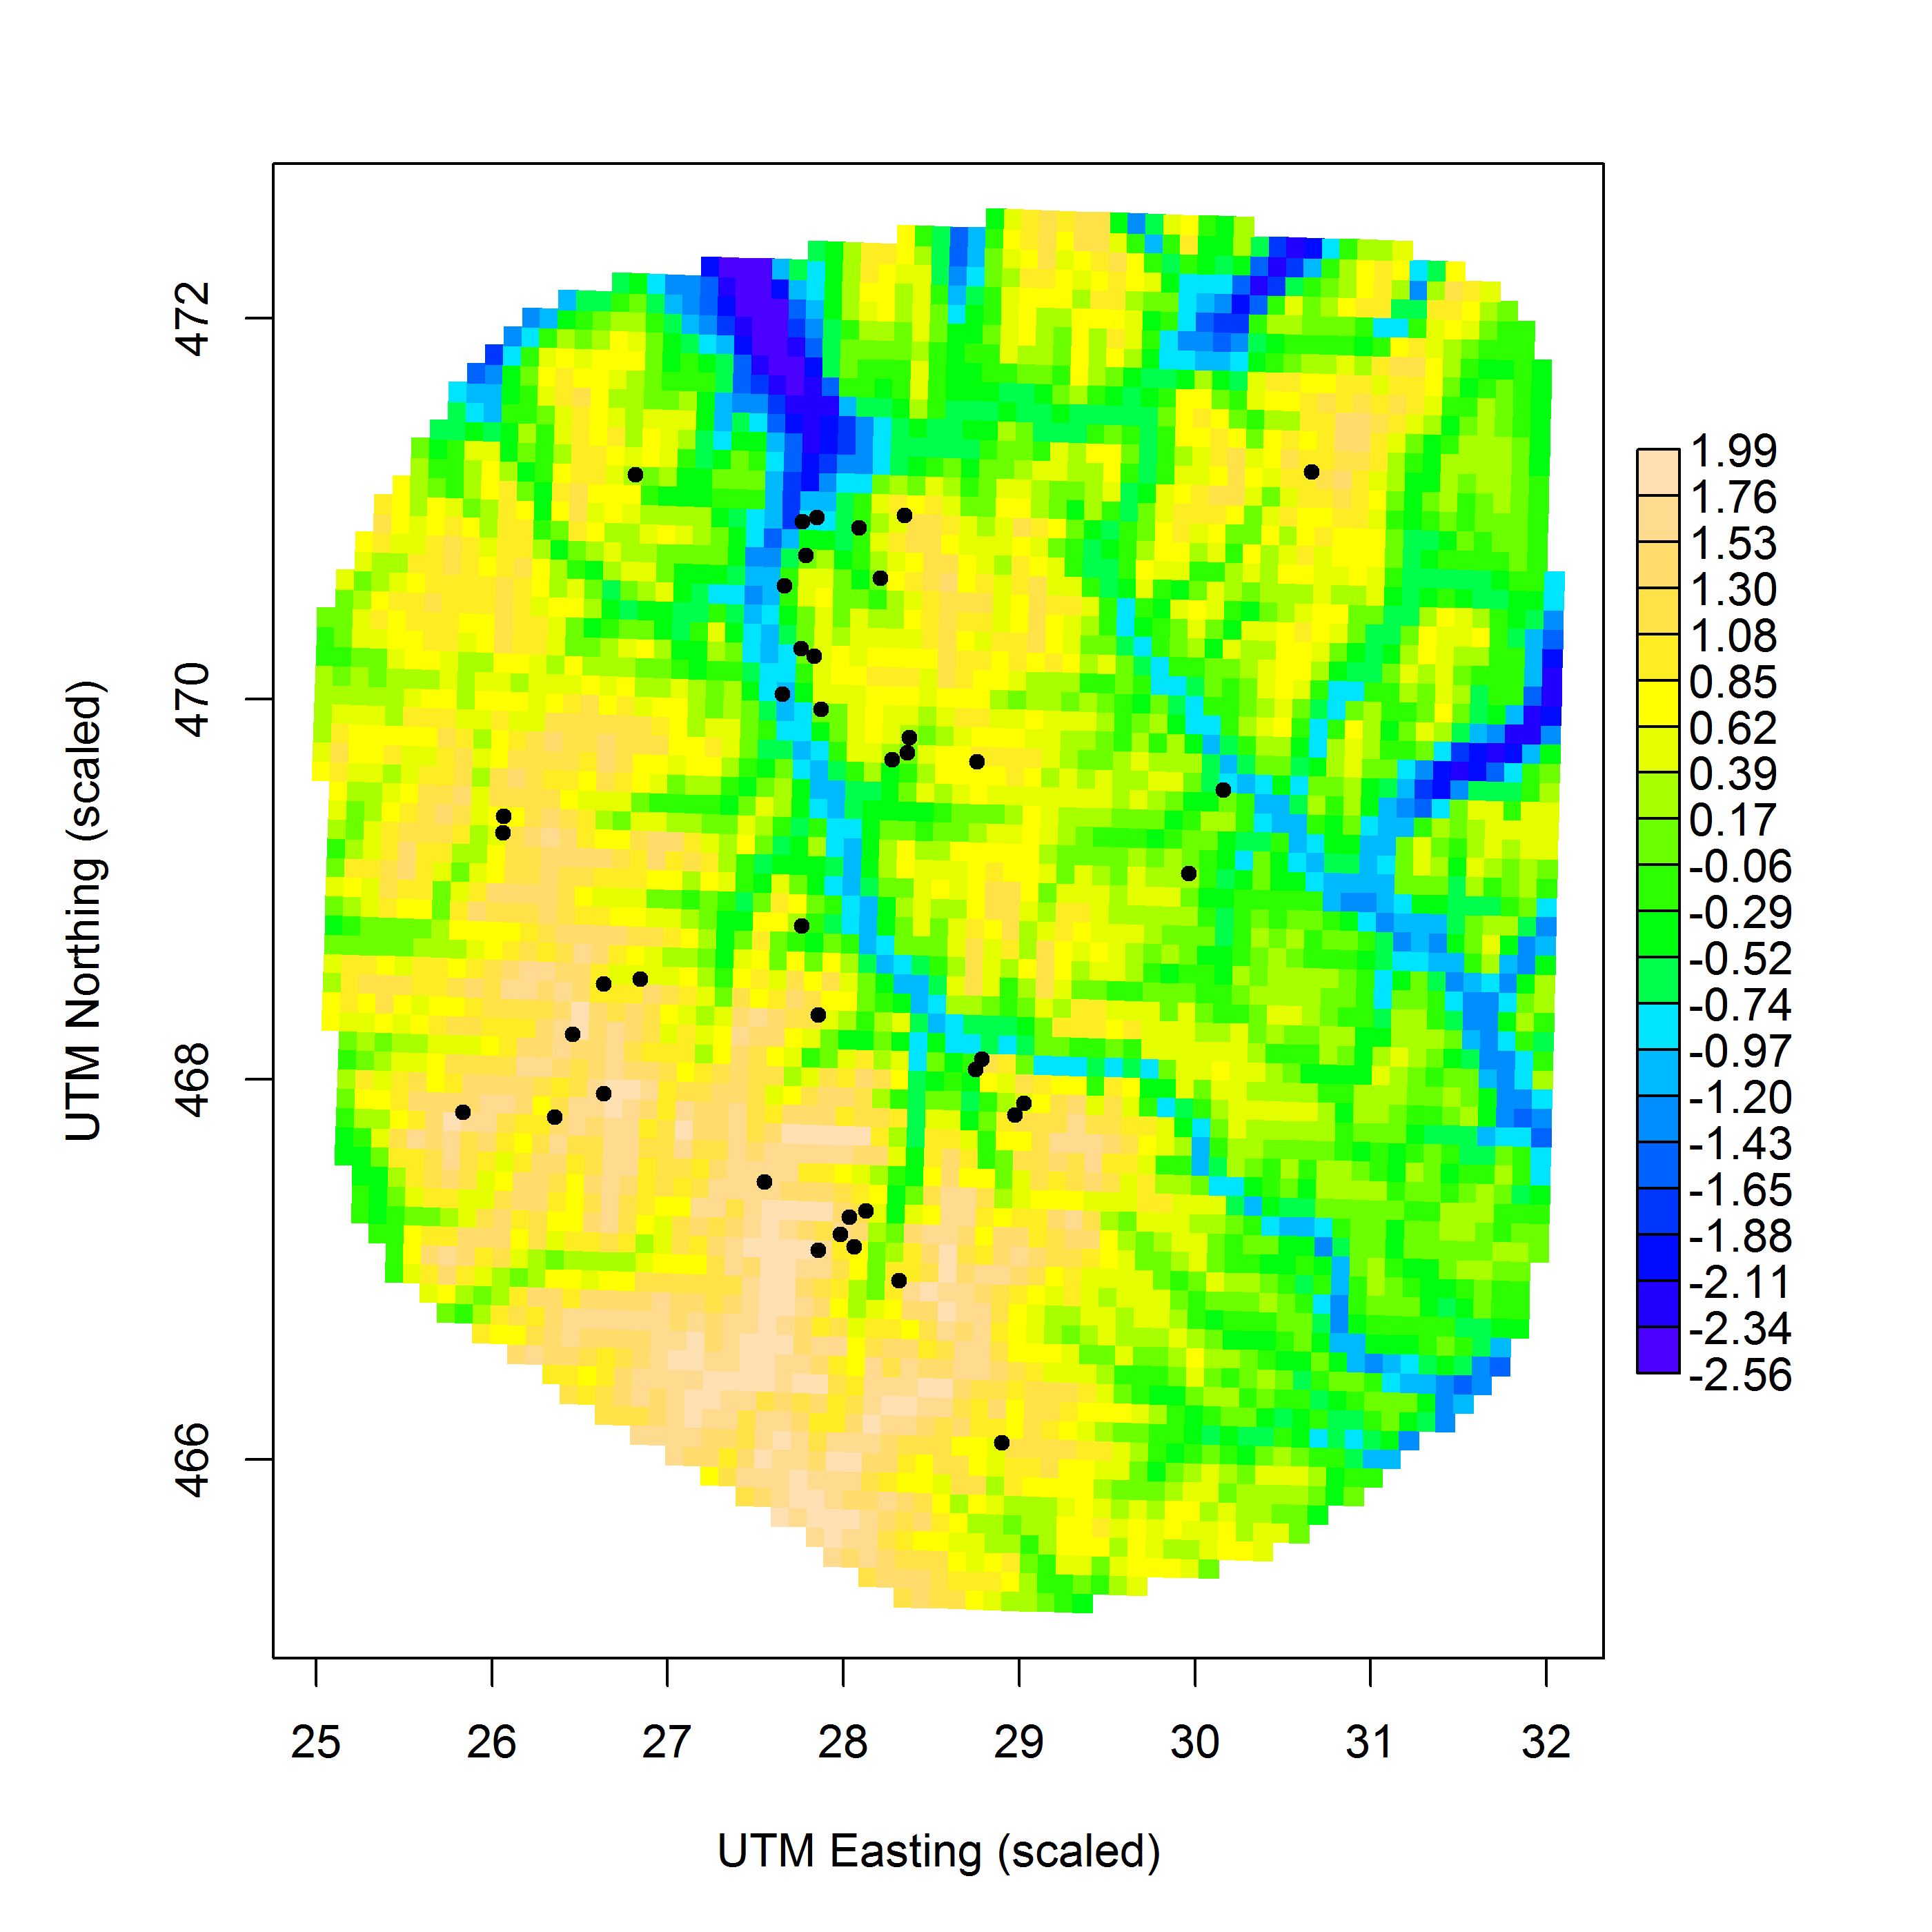
\includegraphics[width=3.5in,height=3.5in]{Ch13-RSF/figs/elev_captures2.png}
\caption{
Elevation (standardized) and location of bear captures.
Multiple captures at a trap location are offset by adding
random noise.
{\bf XXXXXX include trap locations on this figure
see \mbox{\tt ?nybears} and modify that script  XXXXXXXXXXXXXXXXXXXX}
}
\label{fig.elevation}
\end{figure}

A number of models were fitted by \citet{royle_etal:2012mee} which are
reproduced in the
help file \mbox{\tt ?nybears}. The various models are
 based on the Gaussian hazard model
including an ordinary SCR model with no covariates or telemetry data,
the SCR model with elevation affecting either $\lambda_{0}$ or density
$D({\bf x})$ (Chapt. \ref{chapt.state-space}), and models that use
telemetry data.  The 6 models fitted were:
\begin{itemize}
\item[] Model 1: SCR -- ordinary SCR model
\item[] Model 2: SCR+p(C) -- ordinary SCR model with elevation as a
  covariate on baseline encounter probability $\lambda_{0}$.
\item[] Model 3: SCR+D(C) -- ordinary SCR model with elevation as a
  covariate on density only.
\item[] Model 4: SCR+p(C)+D(C) -- ordinary SCR model with elevation as
  a covariate on both baseline encounter probability and density.
\item[] Model 5: SCR+p(C)+RSF -- SCR model including data from 3
  telemetered individuals.
\item[] Model 6: SCR+p(C)+RSF+D(C) -- SCR model including telemetered
  individuals and with elevation as a covariate on density.
\end{itemize}
Its tempting to want to compare these different models by AIC but,
because models 5 and 6 involve additional data, they cannot be
compared with models 1-4.
Parameter
estimates are shown in Table \ref{tab.nyresults} (reproduced from
\citet{royle_etal:2012mee}).



{\bf xxxx below is exactly plagarized from the paper}

Looking at  models 1-4, which do not use the telemetry observations,
models in which elevation effects density are preferred, and we see a
a large positive response to elevation, which is apparent in
consistent with the visual pattern apparent in
Fig. \ref{fig.elevation} (more captures at higher elevations).
Conversely,
there is a negative effect of elevation on
space usage (the parameter $\alpha_{2}$).
The estimate of $N$ for the 4600 km$^2$ state-space, based on the best
model is about 103 bears $(\exp(4.25)+33)$.
In the two models that include the additional telemetry data, a couple
points stand out: Clearly the elevation effect on density is
important, reducing the negative log-likelihood by 5 units. The effect
of elevation on density and space usage are roughly consistent with
Model 4 which did not use telemetry data. Furthermore, the standard
errors (SE) of those two parameter estimates are reduced considerably
when the model uses telemetry data, as is the SE for estimating
$\log(\sigma)$.  The SE for estimating $\log(n_{0})$ is only improved
incrementally compared to the models without telemetry data.  We used
the best model, \mbox{\tt SCR+p(C)+RSF+D(C)}, to produce a map of
density (Fig. \ref{fig.density}) which shows clearly the pattern
induced by elevation. We also produced a map
(Fig. \ref{fig.spaceusage}) to illustrate the effect of elevation on
space usage. This shows the relative probability of using a pixel
${\bf x}$ relative to one of mean elevation, and of the same distance
from an individual's activity center.
% remind people how to compute "the relative prob of using pixel x XXXX
%The cool thing about these models is we can make pretty
%multi-colored maps of things.  A map of density under the
%model is shown in fig. \ref{fig.density}.  A map of space usage in
%terms of the relative probability of using pixel $x$ relative to the
%average pixel is shown in Fig. \ref{fig.spaceusage}.


\begin{table}
\centering
\caption{
Summary of model-fitting results for the black bear study. Parameter
estimates are $\alpha_{0} = \log(\lambda_{0})$ and $\sigma$ is the
scale parameter of the half-normal hazard rate encounter model.
The SCR data are based on $n=33$ individuals, and the telemetry data
are based on 3 individuals.
{\bf XXXXX Redo this table. convert log(n0) to N.hat XXXXX}
}
\begin{tabular}{c|rrrrrr}
\hline \hline
model         & $\alpha_0$ & $\log(\sigma)$ & $\alpha_{2}$ & $\log(n_{0})$ &
$\beta$       & -loglik                                                                         \\ \hline
SCR+p(z)      & -2.8600    & -1.1170        & 0.1750       & 4.1400        &        & 122.7380  \\
   SE         & 0.3899     & 0.1390         & 0.2478       & 0.3657        &        &           \\
 SCR          & -2.7290    & -1.1220        & ---          & 4.1100        &        & 122.9900  \\
   SE         & 0.3454     & 0.1404         &              & 0.3618        &        &           \\
SCR+D(z)      & -2.7150    & -1.1330        & ---          & 4.1140        & 1.2470 & 118.0070  \\
   SE         & 0.3526     & 0.1394         &              & 0.3575        & 0.4083 &           \\
SCR+p(z)+D(z) & -2.4840    & -1.1570        & -0.3840      & 4.2550        & 1.5710 & 117.0750  \\
   SE         & 0.3910     & 0.1421         & 0.2761       & 0.3768        & 0.4630 &           \\
SCR+RSF       & -3.0680    & -0.8140        & -0.2810      & 3.8840        &        & 1271.7390 \\
   SE         & 0.2722     & 0.0364         & 0.1176       & 0.3626        &        &           \\
SCR+RSF+D(z)  & -3.0700    & -0.8100        & -0.3710      & 4.0280        & 1.2730 & 1266.7000 \\
   SE         & 0.2720     & 0.0368         & 0.1239       & 0.3661        & 0.4110 &           \\
\hline
\end{tabular}
\label{tab.nyresults}
\end{table}



\begin{figure}
\centering
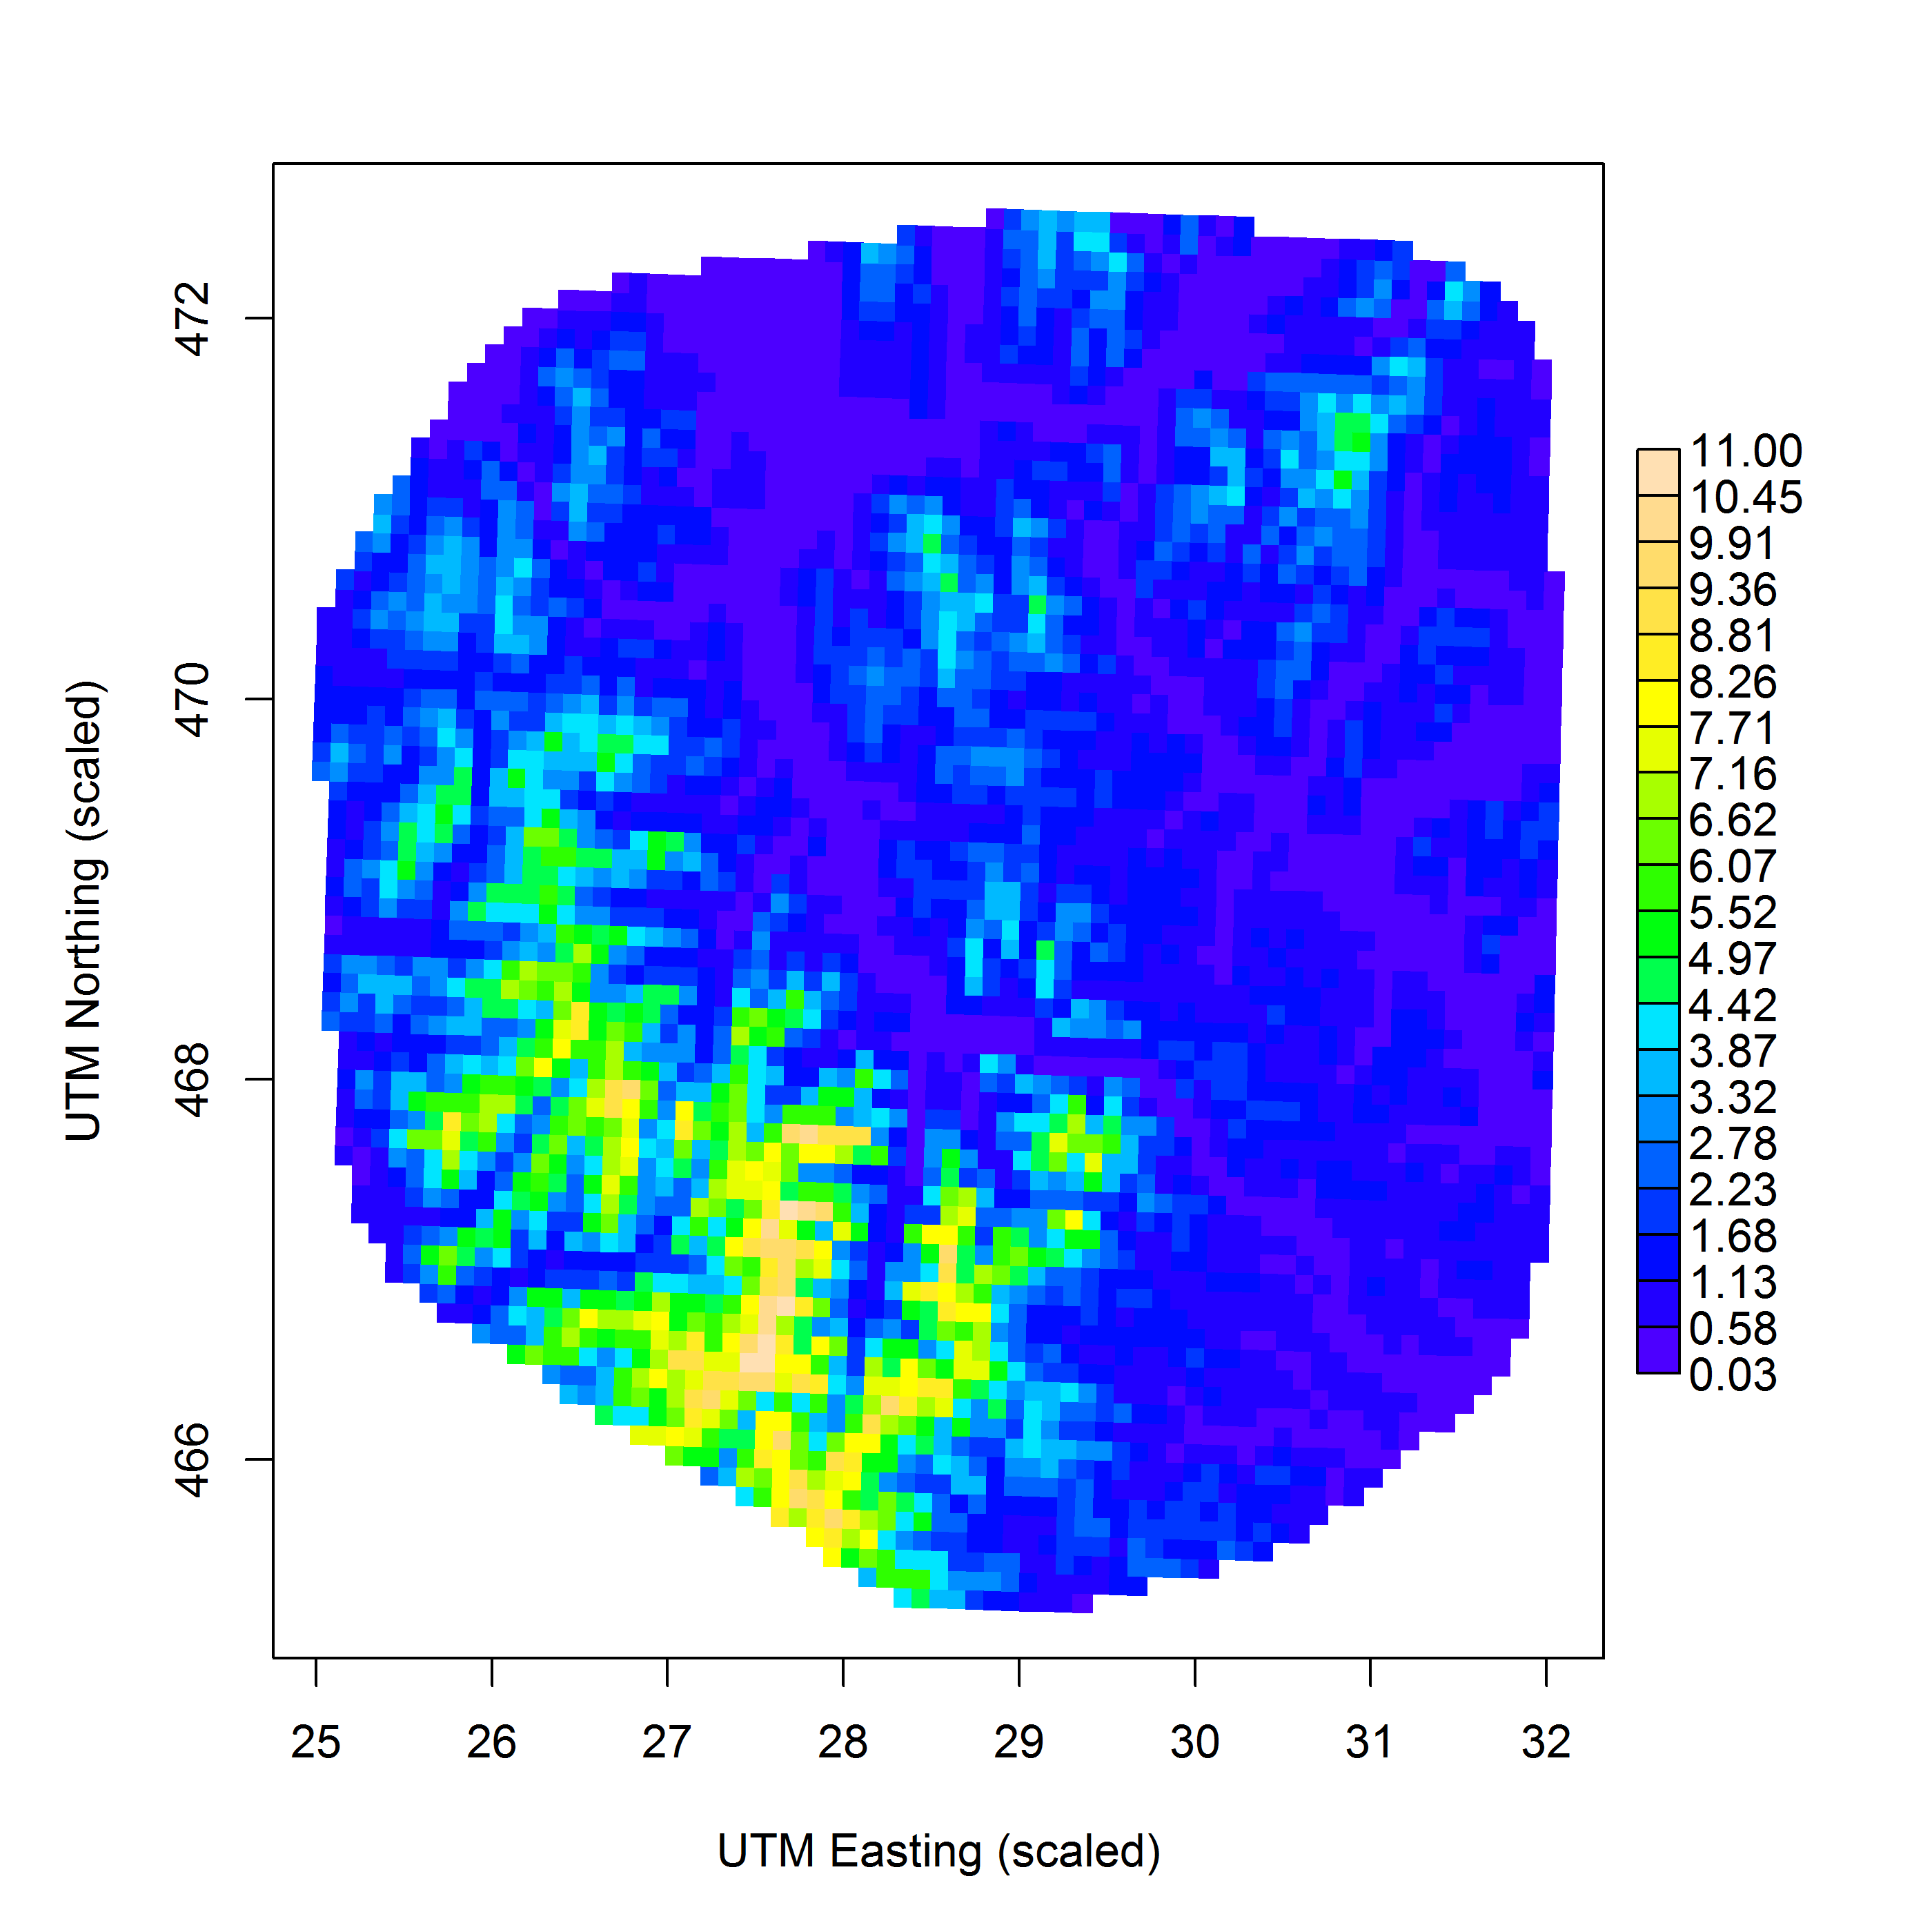
\includegraphics[width=3.5in,height=3.5in]{Ch13-RSF/figs/density2.png}
\caption{Predicted density of black bears (per 100 km$^2$) in central New York study
  area.
}
\label{fig.density}
\end{figure}


\begin{figure}
\centering
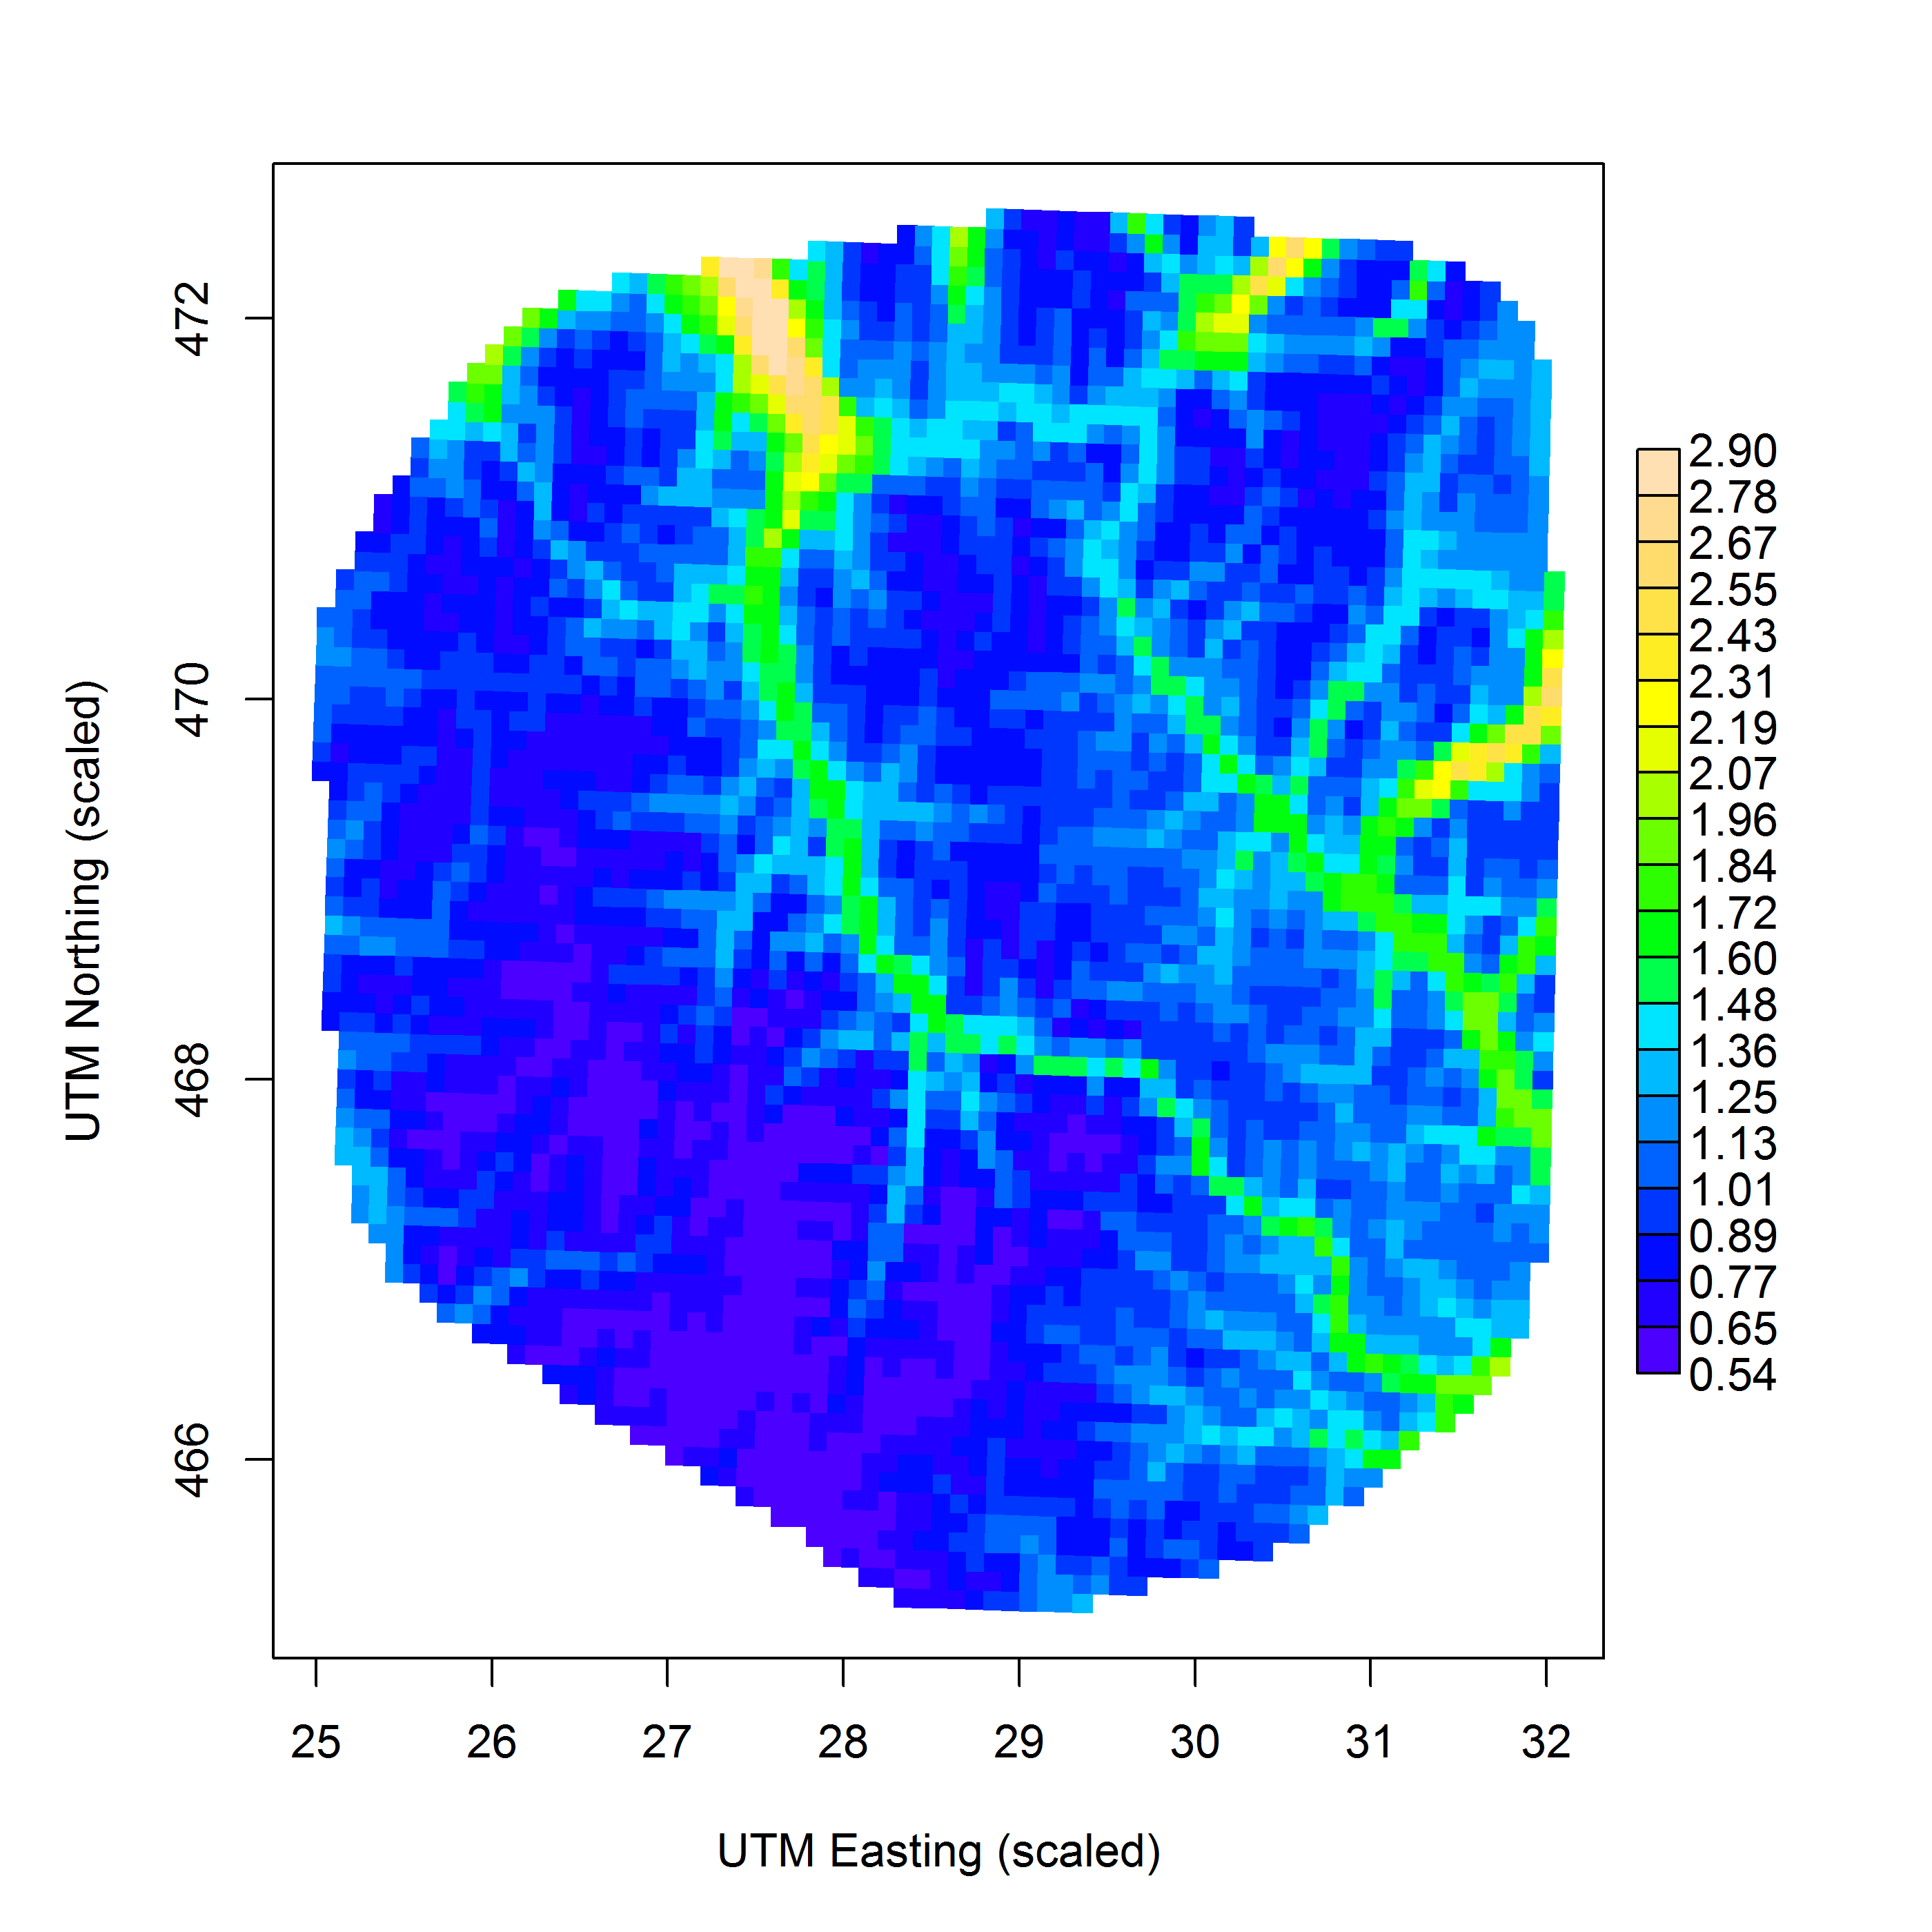
\includegraphics[width=3.5in,height=3.5in]{Ch13-RSF/figs/spaceusage2.png}
\caption{Relative probability of use of pixel ${\bf x}$ compared to a pixel
  of mean elevation, at a constant distance from the activity center.
}
\label{fig.spaceusage}
\end{figure}


The covariate, elevation, appears to affect
 density and space usage
differently.  It was suggested that
density is operating at the second-order scale of resource selection
and ``....is largely related to the spacing of individuals and their
associated home ranges across the landscape.   On the other hand, our RSF was defined
based on selection of resources within the home range (third-order).'' \citep{royle_etal:2012mee}
The positive effect of density to elevation is consistent with some
other studies  \citep[e.g.][]{frary_etal:2011}, and
the negative effect of elevation
on space usage was attributed to seasonal variation in food
availability, usage of corridors, or environmental conditionas.


\section{Simulation Study}

\citet{royle_etal:2012mee} presented results of a simulation study
based on the landscape shown in Fig. \ref{rsf.fig.habitat}, and based
on a population of $N=100$ and $N=200$ individuals with activity
centers distributed uniformly over the landscape, subjected to
encounter over $K=10$ sampling periods, by a $7 \times 7$ array of
trapping devices located on the the integer coordinates $(u*5,v*5)$
for $u,v = 1,2,3,4,5,6,7$. The encounter model and parameter values
were:
\[
\mbox{ cloglog}(p_{ij}) = -2  -\frac{1}{2\sigma^{2}} d_{ij}^{2} + 1 \times C({\bf x}_{j})
\]
for $\sigma =2$. In the absence of the covariate $z$, this corresponds
to an individual having a bivariate normal home range with standard
deviation 2 (Sec. \ref{scr0.sec.implied}).
These settings yielded an average of about $n=61$ individuals captured for
the $N=100$ case and about $n=123$ for the $N=200$ case. The \mbox{\tt
  scrbook} package contains the {\bf R} script for running this
simulation exercise (see \mbox{\tt ?RSFsim}). Table 2 in Royle et
al. (expanded in Table XXX below) showed a pretty dramatic bias in estimating $N$ if the covariate
is omitted from the analysis. You don't need telemetered guys but you
do need the covariate.... this is a key point.......  $\sigma$ is only
slightly biased, however. The covariate effect $\alpha_{2}$ is
estimated unbiasedly when we use RSF data or when we use it as a
covariate in the encounter model alone.

\begin{table}[ht]
\centering
\caption{To check misspecification with isotropic h/r model I refitted the N =
200 cases and fit the SCR only and SCR/RSF models IN ADDITION to the
SCR0 model with isotropic encounter model.}
\caption{in the paper:
Mean and RMSE of sampling distribution of the MLE of $N$ and
  other model parameters under a model of resource selection using
  only SCR data, SCR combined with RSF data on $N_{tel}$ individuals,
  and with RSF only data on $N_{tel}$ individuals. Simulations results
  are based on 500 Monte Carlo simulations of populations containing
  $N=100$ or $N=200$ individuals. The true parameter values were
  $\alpha_{2} = 1$ and $\sigma = 2$.
}
\begin{tabular}{ccccccc}
        &  Nhat &RMSE   &  ahat &RMSE  & sighat & RMSE    \\
n=2     &       &       &       &      &        &         \\
SCR+C(x)& 199.11&  14.28&  0.99 &  0.09&   2.00 &  0.090  \\
SCR+RSF & 199.11&  13.80&  0.99 &  0.09&   2.00 &  0.079  \\
SCR0    & 161.48&  39.98&   --  &   -- &   1.84 &  0.180  \\
n=4   &       &      &        &    &        &          \\
SCR only 199.67  13.87   1.00   0.09   2.00   0.090
SCR/RSF  199.65  13.59   1.00   0.09   2.00   0.072
SCR0     161.32  40.00    --     --    1.83   0.191

n=8    &       &      &        &    &        &          \\
SCR only 199.24  15.49   0.99   0.10   2.01   0.093
SCR/RSF  199.55  14.17   0.99   0.08   2.00   0.063
SCR0     161.46  40.06    --     --    1.84   0.184

n=12    &       &      &        &    &        &          \\
SCR only 200.41  15.16   0.99   0.10   2.00   0.086
SCR/RSF  200.95  13.04   1.00   0.08   2.00   0.051
SCR0     162.40  38.95    --     --    1.84   0.185
n=16     &       &      &        &    &        &          \\
SCR only 199.16  15.62   1.00   0.09   2.00   0.095
SCR/RSF  199.63  13.38   1.00   0.07   2.00   0.052
SCR0     160.93  40.44    --     --    1.84   0.190
\end{tabular}
\end{table}





\begin{comment}
{\small
\begin{verbatim}
N=100, 300 iters each, mean SCR only N: 99.418     N=200, 500 iters. Mean SCR only N = 199.712
n=2          Nhat RMSE  ahat RMSE  sighat  RMSE    Nhat RMSE  ahat RMSE  sighat  RMSE
SCR only:   99.73  9.97  0.99  0.14  2.00  0.124  198.85  14.24   0.99   0.10   2.00   0.091
SCR/RSF:    99.94  9.54  0.99  0.12  2.00  0.097  199.37  12.80   0.99   0.09   2.00   0.078
sbar        98.89  9.50  0.93  0.14  1.97  0.100  197.87  13.94   0.96   0.10   1.99   0.080
RSF only     --    --    1.03  0.33  2.00  0.160    --      --    1.04   0.33   1.99   0.169
n=4
SCR only    99.10  9.83  0.99  0.13  2.00  0.127  200.06  15.34   1.00   0.09   2.00   0.092
SCR/RSF     99.17  9.47  0.99  0.11  2.00  0.086  200.25  14.36   1.00   0.08   2.01   0.073
sbar        97.43  9.68  0.89  0.16  1.97  0.090  198.14  14.31   0.94   0.10   1.98   0.075
RSF only     --     --   0.98  0.22  2.00  0.119    --     --     1.02   0.21   2.01   0.122
n=8
SCR only    99.59 10.00  1.00  0.13  2.00  0.130  200.85  14.06   1.00   0.09   2.00   0.087
SCR/RSF     98.90 10.02  0.99  0.10  2.00  0.071  200.29  13.98   1.00   0.08   2.00   0.061
sbar        96.07 10.37  0.84  0.19  1.96  0.078  196.46  14.59   0.90   0.13   1.97   0.069
RSF only     --    --    0.98  0.16  2.01  0.084    --     --     0.99   0.16   2.00   0.084
n=12
SCR only    99.44 10.73  0.98  0.13  2.02  0.128  198.76  14.47   0.99   0.10   2.00   0.091
SCR/RSF     99.96 10.26  1.00  0.09  2.00  0.059  198.72  14.14   1.00   0.08   2.00   0.054
sbar        96.30 10.49  0.82  0.20  1.96  0.071  193.83  15.14   0.87   0.15   1.97   0.063
RSF only     --    --    1.01  0.12  2.00  0.069    --     --     1.01   0.13   2.00   0.069
n=16
SCR only    99.23 10.74  0.99  0.14  2.00  0.128  200.04  14.09   0.99   0.10   2.01   0.088
SCR/RSF     99.20  9.79  1.00  0.09  1.99  0.057  200.25  13.40   1.00   0.07   2.00   0.047
sbar        95.10 10.17  0.80  0.22  1.95  0.075  194.38  14.26   0.85   0.17   1.96   0.059
RSF only     --    --    1.00  0.10  1.99  0.061    --     --     1.00   0.11   2.00   0.055
\end{verbatim}
}
\end{comment}


Royle et al., looked at the MLE performance under SCR+telemetry
designs having
 2, 4, 8, 12, and 16 telemetered individuals, with 20
independent telemetry fixes {\it per} individual, assuming
individuals were using space according to a RSF model with the same
parameters as those generating the SCR data.
They fitted 3 models: (i)
the SCR only model, in which the telemetry data were not used; (ii)
the integrated SCR/RSF model which combined all of the data for
jointly estimating model parameters; and (iii) the RSF only model
which just used the telemetry data alone (and therefore $\alpha_{0}$
and $N$ are not estimable parameters).  The focus of the simulations
was to address the following basic questions: (1) how much does the
root mean-squared error (RMSE) of $\hat{N}$ improve as we add or
increase the number of telemetered individuals?  (2) How well does the
SCR model do at estimating the parameter of the RSF with {\it no}
telemetry data?  (3) How much does the precision of the RSF parameter
improve if we add SCR data to the telemetry data?

Estimators unbiased pretty much.
In terms of RMSE of the MLEs, generally there is about a 5\% reduction
in RMSE when we have at least 2 telemtered individuals,
and, although
there is a lot of MC error in the RMSE quantities, it might be as much
as a 10\% reduction (tops) as $n$ increases under the higher $N=200$ setting. This makes sense because
we nail down the parameters and still don't know where guys are, and
get info about mean p, i.e. $\alpha_{0}$, only from the SCR data. Thus
estimating $N$  benefits only slightly from the addition of telemetry
data.

Estimating the RSF parameter $\alpha_{2}$ exhibits negligible or no
bias except when ${\bf s}$ is estimated and, interestingly, it is
well-estimated from SCR data alone and even better than RSF data alone
(in terms of RMSE) until we have more than 200 or so telemetry
observations.  The big improvement comes in esetimating the home range
parameter $\sigma$ which is unbiased except when we estimate ${\bf s}$
in which case it exhibits only modest bias.  However, there is huge
improvement in RMSE of $\hat{\sigma}$, perhaps as much as 50-60\% in
some cases, but that really doesn't translate much into esetimating
$N$.  Improvement due to adding RSF data from telemetry diminishes as
the expected sample sizes increases, and so telemetry data does less
to improve the precision of
$\hat{\sigma}$ and $\hat{\alpha}_{2}$
for $N=200$ than for $N=100$.




\begin{verbatim}

Results for $N=100$, $N=200$ and $N_{tel}=(2,4,8,12,16)$ are presented
in Table \ref{tab.results1}. We note that the first row of each batch
(labeled ``\mbox{\tt SCR only}'') represent the same estimator and data
configuration. These replicate runs of the SCR-only situation give us
an idea of the inherent Monte Carlo (MC) error in these simulations, which is
roughly about 0.25 and 0.89 on the $N$ scale for the $N=100$ and
$N=200$ cases, respectively.  The mean $N$ for the SCR-only
estimator across all 5 simulations for $N=100$ was
$\mbox{mean}(\hat{N}) = 99.418$, an empirical bias of $0.6\%$. For
$N=200$, the estimated $N$ across all 5 simulations (5 levels of
$N_{tel}$) was $\mbox{mean}(\hat{N}) = 199.712$, an empirical bias of
about $0.15\%$, within the Monte Carlo error of the true value of $N=200$.  The
results suggests a very small bias of $< 1\%$ in the MLE of $N$ for
both the  SCR-only and combined SCR/RSF estimators.  In practice, we
expect a small amount of bias in MLEs as likelihood theory only
guarantees asymptotic unbiasedness.


In terms of RMSE for estimating $N$, we see that (Table
\ref{tab.results1}), generally, there is about a 5\% reduction in RMSE
when we have at least 2 telemetered individuals. And, although there
is a lot of MC error in the RMSE quantities, it might be as much as a
10\% reduction as the sample size of captured individuals increases
under the higher $N=200$ setting. This incremental improvement in RMSE
of $\hat{N}$
makes sense because, while the
telemetry provides considerable information about the structural
parameters of the model, it provides no information about mean $p$,
i.e. $\alpha_{0}$, which comes only from the SCR data. Thus estimating
$N$ benefits only slightly from the addition of telemetry data.


The MLE of the RSF parameter $\alpha_{2}$ exhibits negligible or no
bias under {\it both} the SCR only and SCR/RSF estimators. It is
well-estimated from SCR data alone and even better than RSF data alone
(in terms of RMSE) until we have more than 200 or so telemetry
observations\footnote{This may appear pardoxical, but the SCR study is
  generating more spatial locations of individuals than the telemetry
  study based on 2 or 4 individuals}.  The biggest improvement from the use of telemetry data
comes in estimating the parameter $\sigma$. We see that $\hat{\sigma}$
is effectively unbiased, and there is a very large improvement in RMSE
of $\hat{\sigma}$, perhaps as much as 50-60\% in some cases, when the
telemetry data are used in the combined estimator (that does not
translate much into improvements in estimating $N$ as we saw
previously).  Improvement due to adding telemetry data diminishes as
the expected sample sizes increases, and so telemetry data does less
to improve the precision of $\hat{\sigma}$ and $\hat{\alpha}_{2}$ for
$N=200$ than for $N=100$. This is because the SCR data alone are
informative about both of those parameters.


The results as they concern likelihood estimation of $N$ suggest that
there is not a substantial benefit to having telemetry
data. Estimators ``SCR only'' and ``SCR/RSF'' both appear
approximately unbiased for $N=100$ and $N=200$, and for any sample
size of telemetered individuals. The RMSE is only 5-10\% improved with
the addition of telemetry information.  However, we find that there is
substantial bias in $\hat{N}$ if we use the {\it misspecified} model
that contains no resource selection component. That is, if we leave the
covariate $z({\bf x})$ out of the model and incorrectly fit a model
with a symmetric and spatially constant encounter model, we see about
20\% bias in the estimates of $N$ in our limited simulation study
(Table \ref{tab.bias}). As such, accounting for resource
selection is important, even though, when accounted for, telemetry
data only improves the estimator incrementally.
In addition, we find that the importance of telemetry data is
relatively more important for smaller sample sizes. We carried-out one
simulation study for the $N=100$ case, but with lower average encounter
probabilities, setting $\alpha_{0}=-3$. This produces
relatively smaller data sets with  $E[n] = 37$.
There are some important features evident from
the results depicted in Table \ref{tab.lowp}.
 First, as a result of the small samples, the MLE of $N$ is
biased for both SCR only and SCR/RSF estimators, although less biased
for the SCR/RSF estimator than for SCR only. The persistent bias in
$\hat{N}$ for both models results from the information about
$\alpha_{0}$ coming only from SCR data, and that estimator itself is
intrinsically biased in small samples.  Conversely, the estimator of
$\alpha_{2}$, the RSF parameter, appears unbiased for all 3 estimators
(SCR only, SCR/RSF and RSF only), as does the estimator of $\sigma$.
We see relatively larger improvements in RMSE (compared with Table
\ref{tab.results1}) of $\hat{N}$, and those improvements
increase substantially as $N_{tel}$ increases.
\end{verbatim}


\section{Relevance and Relaxation of Assumptions}


In constructing the combined likelihood for RSF and SCR data, we
assumed the data from capture-recapture and telemetry studies were
independent of one another. This implies that whether or not an
individual enters into one of the data sets has no effect on whether
it enters into the other data set.  We cannot foresee situations in
which violation of this assumption should be problematic or invalidate
the estimator under the independence assumption.  In some cases it
might so happen that some individuals appear in {\it both} the RSF and
SCR data sets. In this case, ignoring that information should entail
only an incremental decrease in precision because a slight bit of
information about an individuals activity center is disregarded.
\begin{comment}
If
individuals that have telemetry instructments can also be encountered
in traps (and properly identified), then it would be possible to
modify the combined likelihood so that the individual activity centers
is preserved across both hunks of the likelihood.  In such cases where
we can match some individuals between the two samples, regarding them
as independent should only entail a minor loss of efficiency because
we are disregarding more precise information on a small number of
activity centers. Moreover, we believe, it is unlikely in practice to
expect the two samples to be completely reconcilable and that the
independence formulation is the most generally realistic.
\end{comment}

 Our model pretends that we don't know anything
about the telemetered individuals in terms of their encounter history
in traps.  In principle it shouldn't be difficult to admit a formal
reconciliation of individuals between the two lists. In that case, we
just combine the two conditional likelihoods before we integrate ${\bf
  s}$ from the conditional likelihood. This would be almost trivial to
do if {\it all} individuals were reconcilable (or none as in the case
we have covered here) but, in general, we think you will always have
an intermediate case -- i.e., either none will be or at most a subset
of telemetered guys will be known. More likely you have variations of ``well, that
guy looks telemetered but we don't know which guy it is....hmmm'' and
that case, basically a type of marking uncertainty or
misclassification, is clearly more difficult to deal with.
This is related to some of the mark-resign material ({\bf XXXXXXXXXX
chapter 19???? XXXXXXXX}).

We developed the model in a discrete landscape which regarded
potential trap
locations and the covariate $z({\bf x})$ as being defined on the same
set of points. In practice, trap locations may have been chosen
independent of the definition of the raster and this does not pose any
challenge or novelty to the model as we developed it. In that
case, the covariate(s) need to be defined  at each trap location.
The model should be applicable also to covariates that are naturally
continuous (e.g., distance-based covariates) although, in pratice, it
will usually be sufficient to work with a discrete representation of
such covariates.

The multinomial RSF model for telemetry data assumes
independent observations of resource selection.  This would certaintly
be reasonable if telemetry fixes are made far apart in time (or thinned).
However, as noted by \citet{royle_etal:2012mee}, the independence assumption
is {\it not} an assumption of spatially independent movement outcomes
and.
Active resource selection should probably lead to the appearance of
spatially dependent outcomes,
 regardless of how far apart in time the telemetry
locations are.  Even if resource selection observations are dependent,
use of the independence model probably yields unbiased estimators, but
probably under-states the variance.
Development of integrated SCR+RSF models that
accommodate more general models of movement is needed.




\section{Summary and Outlook}


How animals use space is a fundamental interest to ecologists, and
important in the conservation and management of many species.
Normally this is done by telemetry and models referred to as resource
selection functions \citep{manly_etal:2002} but in all of human
history, animal resource selection has {\it never} been studied using
capture-recapture models. Instead, essentially all applicatiosn of SCR
models have focused on density estimation.  However, it is intuitive
that space usage should affect encounter probability and thus it
should be highly relevant to density estimation in SCR
applications. The development in this chapter shows clearly that these
two ideas can be unified within the SCR methodological framework so
that classical notions of resource selection modeling can be
addresssed simultaneous to modeling of animal density. What we find is
that if animal resource selection is occurring, this can be modeled as
covariate on encounter probability, with or without the availability
of auxiliary telemetry data. If telemetry data do exist, we can
estimate parameters jointly by cominbing the two likelihood components
-- that of the SCR data, and that of the telemetry data.



Active resource selection by individuals
induces a type of heterogeneous encounter probability, and this
induces (possibly severe) bias in the estimated population size for a
state-space when default symmetric
encounter probability models are used.
As such, it is important to account for space usage when important
covariates are known to influence space usage patterns.
Aside from properly modeling this selection-induced heterogeneity, integration of RSF data from telemetry with SCR models achieves a
number of useful advances:
First, it
leads to an improvement in our ability to estimate density,
and also an improvement in our ability to estimate parameters of the
RSF function.  As many animal population studies have auxiliary
telemetry information, the ability to incorporate such information
into SCR studies has broad applicability to many studies.  It seems
possible even to estimate density now, with no spatial recaptures,
provided telemetry data are available.
Secondly,
the integrated model
allows for the estimation of RSF model parameters directly from SCR
data {\it alone}.  This establishes clearly that SCR models {\it are}
explicit models of space usage. In our view, this greatly broadens the
utility and importance of capture-recapture studies beyond their
primary historical use of estimating density or population
size. Finally, the formulation of the model from \citet{royle_etal:2012mee}
makes clear that one of the important parameters of SCR
models, that controlling ``home range radius'', is also directly
estimable from telemetry data alone, and certainly its estimation is
greatly improved with even moderate amounts of telemetry data (see
also \citet{sollmann_etal:2012ecol} and \citet{sollmann_etal:inprepjapplecol}.
This should have some consequences in terms of the design of capture-recapture
studies (Chapt. \ref{chapt.design}), especially as it relates to trap spacing.

The simultaneous conduct of telemetry studies with capture-recapture
is extremely common in field studies of animal populations. However,
the simultaneous, integrated analysis of the two sources of data has
not been done.  The new class of integrated SCR/RSF models based on
the \citet{royle_etal:2012mee} model allows investigators to model how
the landscape and habitat influence movement and space usage of
individuals around their home range, using non-invasively collected
capture-recapture data or capture-recapture data augmented with
telemetry data.  This should improve our ability to understand, and
study, aspects of space usage and it might, ultimately, aid in
addressing conservation-related problems such as reserve or corridor
design. And, it should greatly expand the relevance and utility of
spatial capture-recapture beyond simply its use for density
estimation.






























